\fontsize{13}{15}\selectfont
\section{Đặt vấn đề}

Trong gần 30 năm hình thành và phát triển của Internet, Việt Nam được đánh giá là một trong những nước có tốc độ phát triển Internet nhanh nhất thế giới (Nguyễn, 2022). Theo báo cáo Digital Việt Nam 2024 của We Are Social \& Meltwater, vào tháng 1/2024 dân số Việt Nam đạt mức 99,19 triệu người. Trong đó có 78,44 triệu người dùng Internet (chiếm 79,1\% dân số) và 2,70 triệu người dùng mạng xã hội (chiếm 73,3\% dân số) (Siom, 2024). Phương tiện truyền thông xã hội đã trở thành một phần quan trọng trong cuộc sống hàng ngày của mọi người trên khắp thế giới và nó cũng ngày càng được các công ty sử dụng như một phần của chiến lược tiếp thị, dịch vụ khách hàng, nghiên cứu và phát triển (Varga, 2021). Sự phát triển của truyền thông mạng xã hội không chỉ ảnh hưởng đến hành vi của người tiêu dùng ở các hàng hoá mà còn liên quan và rất ảnh hưởng đến ngành dịch vụ du lịch. Bởi vì du lịch là một ngành công nghiệp sử dụng nhiều thông tin, phụ thuộc mạnh mẽ vào hệ thống điện tử Internet để phân phối sản phẩm của mình trên thị trường và giao tiếp với khách hàng (Anna \& Jens, 2014).

Ở Việt Nam, du lịch là ngành kinh tế có đóng góp quan trọng trong việc tạo ra những chuyển biến tích cực đối với sự phát triển của kinh tế, văn hóa, xã hội và quá trình hội nhập quốc tế (Nguyễn, 2022). Hiện nay Du lịch Việt Nam đang trên đà phát triển mạnh mẽ, thu hút số lượng lớn du khách nội địa và du khách quốc tế, đặc biệt là ở nhóm du khách trẻ tuổi. Theo số liệu từ Tổng Cục thống kê, trong năm 2023, số lượt khách du lịch nội địa là 108.200 nghìn lượt người và lượt khách quốc tế đến Việt Nam hơn 12,6 triệu lượt khách (Tổng cục Thống kê, 2024). So với năm 2022, số lượng du khách nội địa tăng 5,8\% và lượt khách quốc tế đến Việt Nam tăng khoảng 244,2\% (Tổng cục Thống kê, 2024).

Sự phát triển của các nền tảng mạng xã hội không chỉ ảnh hưởng đến hành vi tiêu dùng, trao đổi hàng hóa mà còn ảnh hưởng đến ngành dịch vụ du lịch. Bởi lẽ ngành du lịch cần tận dụng mạng xã hội để tiếp cận khách du lịch, quảng bá sản phẩm và dịch vụ. Bên cạnh đó, mạng xã hội cũng ảnh hưởng đến toàn bộ hành trình du lịch của du khách, từ việc bắt đầu lên kế hoạch, đặt vé cho đến khi họ chia sẻ các trải nghiệm của mình sau chuyến đi. Các du khách ngày nay đang dần có xu hướng thay đổi phương tiện tìm kiếm thông tin về điểm đến du lịch từ phương thức truyền thống như sách hướng dẫn du lịch, đại lý du lịch hay lời giới thiệu từ bạn bè sang tự tìm kiếm thông tin trên mạng xã hội ngay tại nhà thông qua các bài quảng cáo, các bài chia sẻ trải nghiệm chuyến đi, … ngay tại nhà của họ mà không cần phải tốn quá nhiều thời gian và chi phí cho việc tìm hiểu thông tin chuyến đi.

Cách tiếp cận và sử dụng mạng xã hội giữa các thế hệ cũng có sự khác biệt rõ rệt. Việc quảng bá và truyền thông về du lịch thông qua mạng xã hội sẽ có hiệu quả hơn so với phương pháp truyền thống đối với khách hàng thuộc thế hệ Gen Z (Ninan, Roy, \& Cheriyan, 2020). Bởi vì đây là nhóm đối tượng sinh ra và lớn lên trong sự phát triển bùng nổ của công nghệ và Internet, do đó, Gen Z có thể dành hơn 4 tiếng để dùng mạng xã hội mỗi ngày. Và Việt Nam là cũng là một nước có tỉ lệ Gen Z sử dụng mạng xã hội cao, điều đó đã ảnh hưởng đến việc sử dụng mạng xã hội của phần lớn sinh viên, và sinh viên Trường Đại học Tôn Đức Thắng cũng không ngoại lệ. Mạng xã hội không chỉ cung cấp thông tin mà còn tạo ra sự tương tác và mối quan hệ giữa người dùng. Việc ứng dụng mạng xã hội vào việc tìm hiểu thông tin điểm đến và quyết định đi du lịch của sinh viên là điều không còn xa lạ. Tuy nhiên, lại không có nhiều bài nghiên cứu đi sâu vào các tác động cũng như các yếu tố ảnh hưởng từ mạng xã hội đến quá trình tìm kiếm thông tin, quyết định lựa chọn điểm đến của sinh viên, kể cả phạm vi nhỏ hơn là sinh viên Trường Đại học Tôn Đức Thắng.

Chính vì vậy, mục đích của nghiên cứu này là phân tích ảnh hưởng của truyền thông MXH đến quyết định đi du lịch của sinh viên Trường Đại học Tôn Đức Thắng thông qua bốn yếu tố là quảng cáo du lịch trên mạng xã hội, độ tin cậy và chất lượng của thông tin, truyền miệng trên mạng xã hội, người có sức ảnh hưởng trên mạng xã hội. Kết quả nghiên cứu nhằm đưa ra những suy nghĩ mang tính khuyến nghị phù hợp cho sinh viên Trường Đại học Tôn Đức Thắng trong sử dụng mạng xã hội hiệu quả để khai thác thông tin về du lịch. 

\section{Nội dung chính}
	\subsection{Khái niệm}
		\subsubsection{Du lịch}
		
		Căn cứ theo Khoản 1, Điều 3 Luật Du lịch Việt Nam năm 2017, định nghĩa du lịch là các hoạt động có liên quan đến chuyến đi của con người ngoài nơi cư trú thường xuyên trong thời gian không quá 1 năm liên tục nhằm đáp ứng nhu cầu tham quan, nghỉ dưỡng, giải trí, tìm hiểu, khám phá tài nguyên du lịch hoặc kết hợp với mục đích hợp pháp khác.
		
		\subsubsection{Truyền thông mạng xã hội}
		
		Theo định nghĩa của Xiang và Gretzel, truyền thông mạng xã hội là các ứng dụng dựa trên nền tảng Internet bao gồm nội dung do người tiêu dùng tạo ra, các ấn tượng trên phương tiện truyền thông và các nền tảng giao tiếp chung cho phép người dùng chia sẻ kinh nghiệm và ý kiến cá nhân với người khác (Xiang \& Gretzel, 2010). Còn theo Sigala và cộng sự, truyền thông mạng xã hội là một không gian ảo, tại đó cho phép người dùng trên toàn thế giới chia sẻ ý tưởng, quan điểm, kinh nghiệm, thông tin và thiết lập các mối quan hệ mới (Sigala \& Christou, 2012). Các nền tảng mạng xã hội như vậy hỗ trợ cho người dùng trong việc giao tiếp và tìm nguồn thông tin về các dịch vụ khác nhau (Tsai \& Bui, 2021).
		
		Trong ngành du lịch, mạng xã hội đã trở thành một công cụ quan trọng để du khách tiếp cận và truyền tải thông tin du lịch nhau (Tsai \& Bui, 2021). Ảnh hưởng của mạng xã hội đối với khách du lịch có thể được nhìn thấy qua hai chiều: trước khi du lịch và sau khi du lịch. Trước chuyến đi, mọi người tìm kiếm thông tin du lịch và các khuyến nghị chủ yếu để lập kế hoạch, tổ chức và lên ý tưởng. Sau chuyến đi, du khách có thể chia sẻ kinh nghiệm, trải nghiệm của họ trên các nền tảng truyền thông xã hội cho khách du lịch khác tham khảo và tương tác với nhau (Oliveira, Araujo, \& Tam, 2020). Trong nghiên cứu này, tác giả chỉ xem xét khía cạnh trước khi đi du lịch của du khách. Khách du lịch sử dụng mạng xã hội để tìm kiếm thông tin khi lập kế hoạch du lịch trong giai đoạn trước chuyến đi (Xiang \& Gretzel, 2010). Trước chuyến đi, khách du lịch tìm kiếm thông tin và đề xuất về khách sạn, nhà hàng, hoạt động, điểm du lịch, sự kiện và hoạt động dịch vụ về đêm, giúp họ có ý định du lịch chắc chắn hơn nhiều dựa trên các đánh giá có sẵn trên các mạng xã hội như Facebook và TripAdvisor.
		
		Hiện tại, quyết định đi du lịch được thúc đẩy bởi nhiều thành phần trên phương tiện truyền thông mạng xã hội: như độ tin cậy của thông tin, sự hài lòng, các thông tin trên mạng xã hội, thái độ khi đi du lịch, truyền miệng giữa các khách du lịch, v.v (Cheunkamon, Jomnokwao, \& Ratanavaraha, 2020). Có nhiều yếu tố cấu thành truyền thông mạng xã hội, quan điểm về các yếu tố của các nhà nghiên cứu khác nhau khi nghiên cứu về lĩnh vực khác nhau như quảng cáo trực tuyến trên mạng xã hội, giá trị cảm nhận (Al-adamat, Al-Gasawneh, \& Sourak, 2020), độ tin cậy của thông tin, số lượng thông tin, sự hữu ích của thông tin (Ninan, Roy, \& Cheriyan, 2020), sự hữu ích, chất lượng thông tin, nhận thức dễ sử dụng, động lực, nhận thức rủi ro, niềm tin người dùng (Odusanya, Aluko, \& Lal, 2020), niềm tin thương hiệu, chất lượng thông tin (McClure \& Seock, 2020), truyền miệng điện tử, độ tin cậy của thông tin, sự thụ hưởng (Tsai \& Bui, 2021), người có sức ảnh hưởng trên mạng xã hội, độ tin cậy của thông tin, thái độ, (Han \& Chen, 2022).
		
		\subsubsection{Các yếu tố của mạng xã hội ảnh hưởng đến quyết định du lịch}
		\begin{enumerate}[label = \alph*)]
			\item Quảng cáo trên mạng xã hội
			
			Trong nghiên cứu của Al-Adamat và cộng sự, việc tiếp thị, quảng cáo truyền thông được sử dụng để tác động đến các điểm đến, quyết định du lịch và lựa chọn sản phẩm của khách hàng. Các nghiên cứu trước đây cho thấy rằng các chiến lược quảng bá trực tuyến cung cấp cho khách hàng thông tin du lịch có liên quan và quyết định mua hàng của họ (Al-adamat, Al-Gasawneh, \& Sourak, 2020). Các doanh nghiệp ngày nay quảng bá sản phẩm của họ không chỉ thông qua các kênh thông thường như tạp chí, bài báo và người giới thiệu cá nhân, mà còn thông qua các nền tảng truyền thông xã hội như Facebook, Zalo, Instagram và Youtube,…Việc sử dụng quảng cáo trên MXH đã trở thành một công cụ truyền thông chiến lược để tác động trực tiếp đến quyết định mua hàng và hành vi mua hàng (Heinrichs \& cs., 2011). Ninan và cộng sự cho rằng quảng cáo truyền thông xã hội có ảnh hưởng có lợi đến quyết định mua hàng của khách hàng và hành vi mua hàng. Để đạt được mục tiêu này, tiếp thị và quảng cáo truyền thông xã hội đòi hỏi phải cập nhật thường xuyên nội dung, cung cấp thông tin bổ sung và thực hiện các chiến thuật quảng cáo để thu hút khách hàng (Navya, Joel, \& Namitha, 2020).\textit{ Trên cơ sở đó, giả thuyết H1 được đề xuất như sau: Quảng cáo trên mạng xã hội có ảnh hưởng đến quyết định đi du lịch của sinh viên Trường Đại học Tôn Đức Thắng.}
			\item Độ tin cậy và chất lượng của thông tin
			
			Thông tin về một sản phẩm hàng hoá hoặc dịch vụ rất cần thiết đối với khách hàng. Khách hàng cảm thấy tin tưởng và mua sản phẩm/sử dụng dịch vụ thông qua các thông tin do nhà sản xuất cung cấp. Các thông tin này phải thật sự hữu ích trong việc sử dụng dịch vụ và mua sắm hàng hoá của họ (Trương, Hồ, \& Lê, 2023). Hiện nay, ngày càng có nhiều dấu hiệu cho thấy cảm nhận của khách hàng về tính hữu ích là một yếu tố tiên lượng chính của quá trình chấp nhận và đưa ra quyết định cuối cùng của khách hàng (Ninan, Roy, \& K. Cheriyan, Influence of Social Media Marketing on the Purchase Intention of Gen Z, 2020). Theo Bae \& cộng sự (2017), độ tin cậy và chất lượng của thông tin được chia sẻ trên MXH ảnh hưởng rất lớn đến các định hướng và lựa chọn du lịch trong tương lai (Sung, Lee, Eung, \& Kil, 2017). Nguồn cung cấp thông tin uy tín tại các trang mạng xã hội ảnh hưởng đến ý định của khách du lịch bắt nguồn từ các đề xuất trực tuyến của bạn bè và người thân, cũng như thông tin và nhận xét được cung cấp bởi các bên thứ ba như những người có ảnh hưởng, những người dùng khác và các công ty du lịch (Berhanu \& Raj, 2020). Theo Yip và Mo, nội dung thông tin du lịch vẫn là vấn đề then chốt trong ý định mua hàng; đặc biệt là môi trường trực tuyến, nếu thông tin có chất lượng cao sẽ làm tăng ý định mua hàng (Wing \& Wing, 2020). \textit{Trên cơ sơ đó, giả thuyết H2 được đề xuất như sau: Độ tin cậy và chất lượng của thông tin có ảnh hưởng đến quyết định đi du lịch của sinh viên Trường Đại học Tôn Đức Thắng.}
			\item Truyền miệng trên mạng xã hội
			
			Truyền miệng qua MXH được gọi là truyền miệng điện tử (Yang, 2017), hay Electronic Word of mouth – eWOM .Với sự bùng nổ của internet, hình thức giao tiếp này ngày càng quan trọng hơn vì trở thành một trong những nguồn thông tin có ảnh hưởng nhất trên Internet (Abubakar \& Mustafa, 2016), đặc biệt là trong các ngành dịch vụ – du lịch (Marios \& Cina, 2013). Truyền miệng điện tử là tất cả những thông tin liên quan đến việc sử dụng hoặc đặc điểm của sản phẩm, dịch vụ và người bán hàng, được truyền tải một cách không chính thức qua Internet (Litvin, E. Goldsmith, \& Pan, 2008). Để nhấn mạnh vai trò của truyền miệng, Daugherty và Hoffman (2014) cho rằng, truyền miệng là nguồn thông tin quan trọng nhất trong ý định mua hàng và hành vi dự định của người tiêu dùng (Terry \& Ernest, 2014). Người tiêu dùng hiện nay xem truyền miệng điện tử là phương tiện đáng tin cậy nhiều hơn so với những phương tiện truyền thống như truyền hình, đài phát thanh, tờ rơi,… Đây cũng là kênh tiếp thị được người tiêu dùng sử dụng rộng rãi, bởi người gửi và người nhận độc lập với thị trường, khiến cho khách hàng có sự tin cậy cao hơn (Brown, J.Broderick, \& Lee, 2007). \textit{Giả thuyết H3 được đề xuất như sau: Truyền miệng trên mạng xã hội có ảnh hưởng đến quyết định đi du lịch của sinh viên Trường Đại học Tôn Đức Thắng.}
			\item Người có sức ảnh hưởng trên mạng xã hội
			
			Influencer hay còn gọi là “người gây ảnh hưởng”, bất kỳ người dùng trực tuyến nào đều có khả năng trở thành người có sức tác động đến những đối tượng hoặc thị trường nhất định. Tùy vào hoạt động, tiếng nói, lĩnh vực mà họ đang ở trong, hoặc mục đích dùng mạng xã hội..., mà sẽ có những mức độ ảnh hưởng rộng hẹp khác nhau (Nguyên, Trần, Lưu, Lê, \& Nguyễn, 2022). Những người có ảnh hưởng là những người viết nhật ký trực tuyến (blog) hoặc đăng ý kiến của họ trên Youtube, Snapchat, Instagram hay các kênh truyền thông xã hội khác. Điều cốt lõi là họ có cộng đồng riêng trên mạng xã hội và họ sẵn sàng sản xuất nội dung được tài trợ và sản xuất chuyên nghiệp cho những người theo dõi họ (Dương, Nguyễn, Nguyễn, Nguyễn, \& Trần, 2023). Ngày nay, cùng với sự thay đổi trong phương thức giao tiếp và sự hiện diện ngày càng đông đảo của khách hàng trên những nền tảng mạng xã hội trực tuyến, người có ảnh hưởng không chỉ là người nổi tiếng trong một số lĩnh vực đặc thù mà mở rộng thêm là “người sáng tạo nội dung” (content creator). Họ là những chuyên gia tạo ra bất cứ nội dung nào mà người tiêu dùng tương tác, giúp các thông điệp lan truyền rộng rãi hơn trên phương tiện truyền thông xã hội (Campbell \& Justine, 2020). \textit{Giả thuyết H4 được đề xuất như sau: Người có sức ảnh hưởng trên mạng xã hội có ảnh hưởng đến quyết định đi du lịch của sinh viên Trường Đại học Tôn Đức Thắng.}
			
			Dựa trên các lập luận, cơ sở lý thuyết, nghiên cứu đi trước, tác giả đã đưa ra mô hình và giả thuyết nghiên cứu các yếu tố ảnh hưởng đến quyết định đi du lịch của sinh viên Trường Đại học Tôn Đức Thắng xây dựng thông qua 04 yếu tố chính: Quảng cáo du lịch trên mạng xã hội, độ tin cậy và chất lượng của thông tin, truyền miệng trên mạng xã hội, người có sức ảnh hưởng trên mạng xã hội (Trương, Hồ, \& Lê, 2023).
			
				\begin{figure}[H]
					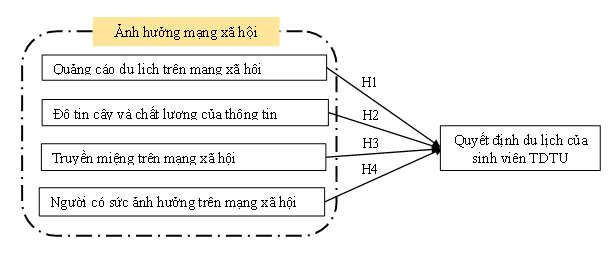
\includegraphics[width=\linewidth]{picture/mo_hinh_de_xuat_nghien_cuu.png}
					\caption{Mô hình đề xuất nghiên cứu}
					\label{mo_hinh_de_xuat_nghien_cuu}
					\centering
				\end{figure}
		\end{enumerate}
			
	\subsection{Lý thuyết nghiên cứu}
		\subsubsection{Lý thuyết hành vi dự định (Theory of Planned Behavior)}
		
		Lý thuyết hành vi dự định (TPB-Theory of Planned Behavior) của Ajzen (1991) được phát triển và cải tiến từ Lý thuyết hành động hợp lý (Theory of Reasoned Action  – TRA). TPB được xem là một lý thuyết quan trọng trong nghiên cứu tâm lý xã hội, cung cấp lời giải thích cho hành vi của con người trong nhiều bối cảnh khác nhau. Theo Ajzen (1991), mô hình TPB dự đoán hành vi bao gồm có các thành phần như sau: Thái độ; Chuẩn chủ quan; Kiểm soát hành vi cảm nhận; Xu hướng hành vi và Hành vi thực sự (hình \ref{mo_hinh_ly_thuyet_hanh_vi_du_dinh})(Ajzen, 1991).
		
		\begin{figure}[H]
			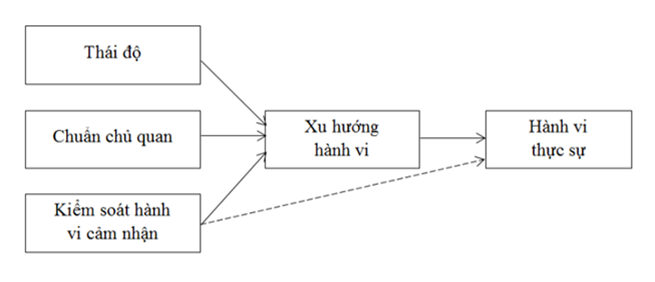
\includegraphics[width=\linewidth]{picture/mo_hinh_ly_thuyet_hanh_vi_du_dinh.png}
			\caption{Mô hình lý thuyết hành vi dự định}
			\label{mo_hinh_ly_thuyet_hanh_vi_du_dinh}
		\end{figure}
		
		\begin{enumerate}[label= (\arabic*)]
			\item “Thái độ đối với hành vi” - Attitude toward the Behavior được định nghĩa là mức độ đánh giá cảm xúc của cá nhân khi thực hiện một hành vi là tích cực hay tiêu cực. Thái độ thường được hình thành bởi niềm tin của cá nhân về hậu quả của việc tham gia thực hiện một hành vi cũng như kết quả của hành vi đó. 
			\item “Chuẩn chủ quan” - Subjective Norms có thể hiểu là áp lực xã hội đến từ sự kỳ vọng của các chủ thể bên ngoài (gia đình, bạn bè, đồng nghiệp...) tác động lên cá nhân dẫn đến thực hiện hành vi nhằm đáp ứng mong đợi hoặc tránh bị phán xét của mọi người xung quanh. Là một trong những yếu tố khuyến khích ý định hành vi liên quan đến hoạt động du lịch.
			\item “Nhận thức kiểm soát hành vi” - Perceived Behavioral Control là chỉ mức độ nhận thức của một cá nhân về sự dễ dàng hoặc khó khăn trong việc thực hiện hành vi cụ thể. Nhận thức về kiểm soát hành vi đã được chứng minh là một yếu tố quan trọng quyết định ý định du lịch (Martin , Martin, \& Ramamonjiarivelo, 2011).
			\item “Xu hướng hành vi” được coi là yếu tố dự đoán tốt nhất về hành vi (Fishbein \& Ajzen, 1975); (Im, Seongtae, \& Kang, 2011); (Martins, Oliveira, \& Popovič, 2014). Các nghiên cứu về mối quan hệ giữa ý định hành vi và việc sử dụng thực tế đã được thực hiện trong lĩnh vực du lịch, ngân hàng trực tuyến và sử dụng dịch vụ di động (Arenas-Gaitan, Peral, \& Jerónimo, 2015); (Baptista \& Oliveria, 2015); (Escobar-Rodríguez \& Carvajal-Trujillo, 2014).
			\item “Hành vi thực sự” là những hành động của cá nhận thực hiện trong thế giới thực dựa trên tác động của các thành phần trên.
			
		\end{enumerate}
		
		\subsubsection{Lý thuyết chấp nhận công nghệ (Theory of Technological Acceptance Model)}
		
		Davis (1989) đã đề xuất Mô hình Chấp nhận công nghệ (TAM – Technology Acceptance Model) (Davis, Bagozzi, \& Warshaw, 1989), dựa trên Lý thuyết hành động lý trí (TRA) (Ajzen, 1991) và Lý thuyết hành vi có kế hoạch (TPB). TAM tập trung vào việc giải thích tại sao cá nhân chấp nhận hoặc từ chối công nghệ thông tin, và đã trở thành một mô hình được áp dụng rộng rãi và được người dùng chấp nhận và sử dụng. Trong TAM, tác giả nhấn mạnh rằng ý định sử dụng có mối liên hệ đáng kể với việc sử dụng thực tế của công nghệ. Ý định được coi là yếu tố quan trọng trong việc sử dụng công nghệ, trong khi các yếu tố khác ảnh hưởng vào việc sử dụng một cách gián tiếp thông qua ý định sử dụng. Tác giả cũng lập luận rằng cảm nhận về độ dễ sử dụng ảnh hưởng đến sự hữu ích của công nghệ, dẫn đến hiệu quả trong công việc khi sử dụng công nghệ. Tuy nhiên, thái độ, như được Mathieson (1991) và Xu et al. (2014) chứng minh, được xem là một biến số ít quan trọng hơn trong mô hình TAM gốc do tác động trung gian yếu của nó đối với niềm tin và ý định sử dụng (Xu, Huang, \& Li, 2019). Do đó, cho đến nay, nhiều nhà nghiên cứu đã đơn giản hóa mô hình TAM để chỉ bao gồm hai yếu tố chính ảnh hưởng trực tiếp đến ý định sử dụng: cảm nhận sự hữu ích và cảm nhận độ dễ sử dụng (hình \ref{mo_hinh_ly_thuyet_chap_nhan_cong_nghe}).
		
		\begin{figure}[H]
			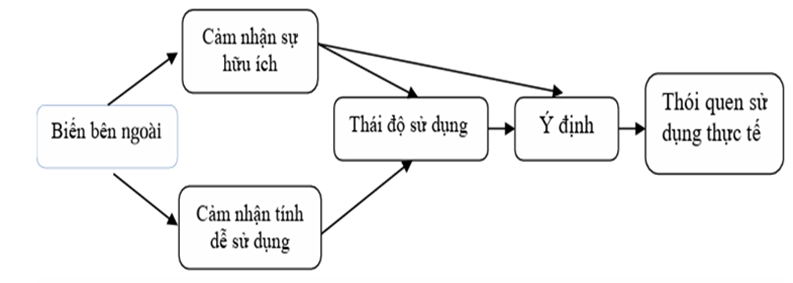
\includegraphics[width=\linewidth]{picture/mo_hinh_ly_thuyet_chap_nhan_cong_nghe.png}
			\caption{Mô hình lý thuyết chấp nhận công nghệ}
			\label{mo_hinh_ly_thuyet_chap_nhan_cong_nghe}
		\end{figure}
		
		Biến bên ngoài: là những nhân tố ảnh hưởng đến niềm tin của một người về việc chấp nhận sản phẩm hay dịch vụ. Những biến bên ngoài thường từ hai nguồn là quá trình ảnh hưởng xã hội và quá trình nhận thức, thu thập kinh nghiệm của bản thân. Biến bên ngoài gồm:
		\begin{itemize}[label=+]
		\item Cảm nhận tính hữu ích là mức độ một người tin rằng sử dụng công nghệ mới sẽ cải thiện và nâng cao hiệu quả công việc. 
		\item Cảm nhận tính dễ sử dụng là mức độ mà một người tin rằng có thể sử dụng hệ thống đặc thù mà không cần sự nỗ lực.
		\end{itemize}	
		
		Thái độ sử dụng là cảm giác tích cực hay tiêu cực về việc thực hiện hành vi mục tiêu, đó là nhân tố quan trọng ảnh hưởng tới thành công của hệ thống.
		
	\subsection{Phương pháp nghiên cứu}
		\subsubsection{Phương pháp chọn mẫu}
		
		Trong bài nghiên cứu về ảnh hưởng của mạng xã hội đến quyết định đi du lịch của sinh viên Trường Đại học Tôn Đức Thắng, tác giả và \dots thực hiện chọn mẫu ngẫu nhiên thuận tiện trên công cụ tạo bảng hỏi gồm các thang đo và mục hỏi được mô tả như Bảng 1. Phần thứ nhất của bảng hỏi nhằm thu thập các thông tin về đặc điểm nhân khẩu học của người trả lời, phần thứ hai gồm các mục hỏi đều dựa trên thang đo Likert 5 điểm và khảo sát thông qua Google Form và các kênh truyền thông khác như Zalo, Facebook và email sinh viên do Trường Đại học Tôn Đức Thắng cung cấp nhằm tạo điều kiện thuận lợi và tiết kiệm thời gian nhất cho các đáp viên cũng như nhóm nghiên cứu trong việc tiếp cận, tương tác và trả lời khảo sát.
		
		
	